%!TEX root = paper.tex"`

\section{Background}

\subsection{Notation}
\begin{figure}
\centering
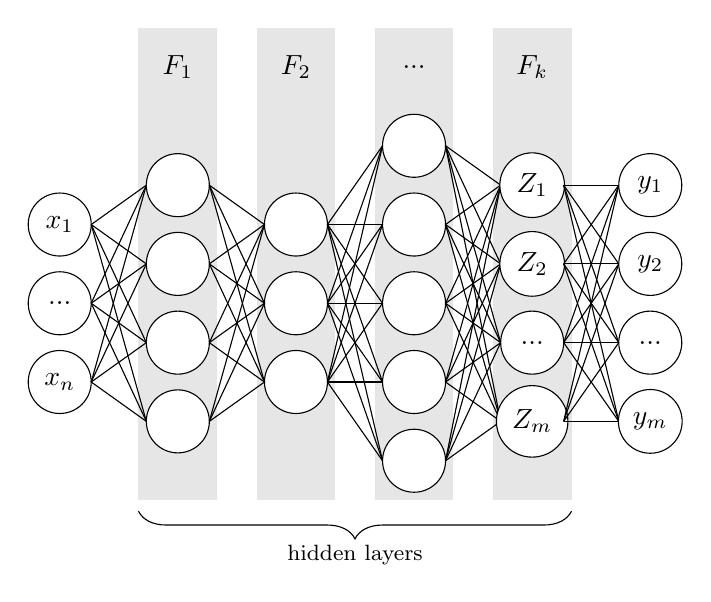
\begin{tikzpicture}[yscale=-1]
\tikzset{neuron/.style={
    shape=circle,
    fill=white,
    draw,
    minimum size=0.8cm
}}

%\draw[step=1cm,gray,very thin,fill=white] (0,0) grid (8,6);

\fill[opacity=0.2,fill=gray] (1,-0.5) rectangle (2,5.5);

\fill[opacity=0.2,fill=gray] (2.5,-0.5) rectangle (3.5,5.5);

\fill[opacity=0.2,fill=gray] (4,-0.5) rectangle (5,5.5);

\fill[opacity=0.2,fill=gray] (5.5,-0.5) rectangle (6.5,5.5);

\node[neuron] at (0, 2) {$x_1$};
\node[neuron] at (0, 3) {...};
\node[neuron] at (0, 4) {$x_n$};

\foreach \x in {1,...,3}{
	\draw (0.4, \x+1) -- (1.1,1.5);	\draw (0.4, \x+1) -- (1.1,2.5);
	\draw (0.4, \x+1) -- (1.1,3.5);
	\draw (0.4, \x+1) -- (1.1,4.5);
}

\node[] at (1.5, 0) {$F_1$};
\foreach \x in {2,...,5}{
	\node[neuron] at (1.5, \x-0.5) {};
	\draw (1.9, \x-0.5) -- (2.6,2);
	\draw (1.9, \x-0.5) -- (2.6,3);
	\draw (1.9, \x-0.5) -- (2.6,4);
}

\node[] at (3, 0) {$F_2$};
\foreach \x in {2,...,4}{
	\node[neuron] at (3, \x) {};
	\draw (3.4, \x) -- (4.1,1);	\draw (3.4, \x) -- (4.1,2);
	\draw (3.4, \x) -- (4.1,3);
	\draw (3.4, \x) -- (4.1,4);
	\draw (3.4, \x) -- (4.1,5);
}

\node[] at (4.5, 0) {...};
\foreach \x in {1,...,5}{
	\node[neuron] at (4.5, \x) {};
	\draw (4.9, \x) -- (5.6,1.5);	\draw (4.9, \x) -- (5.6,2.5);
	\draw (4.9, \x) -- (5.6,3.5);
	\draw (4.9, \x) -- (5.6,4.5);
}

\draw [decorate,decoration={brace,amplitude=10pt,mirror,raise=4pt},yshift=0pt]
(1,5.5) -- (6.5,5.5) node [black,midway,yshift=-0.7cm] {\footnotesize hidden layers};

\node[] at (6, 0) {$F_k$};
\foreach \x in {1,...,2}:
	\node[neuron] at (6, \x+0.5) {$Z_\x$};
\node[neuron] at (6, 3.5) {...};
\node[neuron] at (6, 4.5) {$Z_m$};

\foreach \x in {1,...,4}{
	\draw (6.4, \x + 0.5) -- (7.1,1.5);
	\draw (6.4, \x + 0.5) -- (7.1,2.5);
	\draw (6.4, \x + 0.5) -- (7.1,3.5);
	\draw (6.4, \x + 0.5) -- (7.1,4.5);
}

\foreach \x in {1,...,2}:
	\node[neuron] at (7.5, \x+0.5) {$y_\x$};
\node[neuron] at (7.5, 3.5) {...};
\node[neuron] at (7.5, 4.5) {$y_m$};
\end{tikzpicture}
\caption{Visualization of a neural network}
\label{fig:neuralnetwork}
\end{figure}

\begin{enumerate}
\item Images called Irrbilder by the 
\end{enumerate}